\documentclass[
size=17pt,
paper=smartboard,
mode=present,
display=slidesnotes,
style=paintings,
nopagebreaks,
blackslide,
fleqn]{powerdot}

% styles: sailor, paintings
% wj capsules prettybox
% mode = handout or present


\usepackage{amsmath,graphicx,color,amsfonts}
\usepackage[brazilian]{babel}
\usepackage[utf8]{inputenc}
\newcommand{\palette}{Moitessier}


% palettes:
%    - sailor: Sea, River, Wine, Chocolate, Cocktail 
%    - paintings: Syndics, Skater, GoldenGate, Moitessier, PearlEarring, Lamentation, HolyWood, Europa, MayThird, Charon 

\newcommand{\cursopequeno}{EC01039 CG\underline{PI}}
\newcommand{\cursogrande}{\Large EC01039 -- Computação gráfica e \underline{processamento de imagem}}



\author{Ronaldo de Freitas Zampolo\\FCT-ITEC-UFPA}
\date{2020.2}


\pdsetup{
	lf = {\cursopequeno},
	rf = {Percepção visual}, 
	cf = {\arabic{slide}~/~\pageref*{lastslide}},
	palette = {\palette}, 
	randomdots={false}
}

%opening
\title{\cursogrande\\ \vspace{1cm}Elementos da percepção visual humana}
\author{Ronaldo de Freitas Zampolo\\FCT-ITEC-UFPA}
%\date{ }

\begin{document}
   \maketitle[randomdots={false}]
   \begin{slide}{Agenda}
      \tableofcontents[content=sections]
   \end{slide}

   \section[ slide = true]{O olho humano}
      \begin{slide}[toc=]{A estrutura do olho humano}
         \twocolumn{
         \begin{itemize}
          \item Córnea: tecido transparente que cobre a parte anterior do olho
          \item Esclera: membrana opaca, prologamento da córnea, reveste o restante do olho
          \item Coroide: membrana com rede de vasos, fonte de nutrição para o olho, pigmentado
          \item Íris: controle da quantidade de luz que entra no olho
          \item Pupila: abertura central da íris (2 a 8 mm)
          \item Cristalino: lente adaptável
         \end{itemize}}
         {
         \begin{center}
            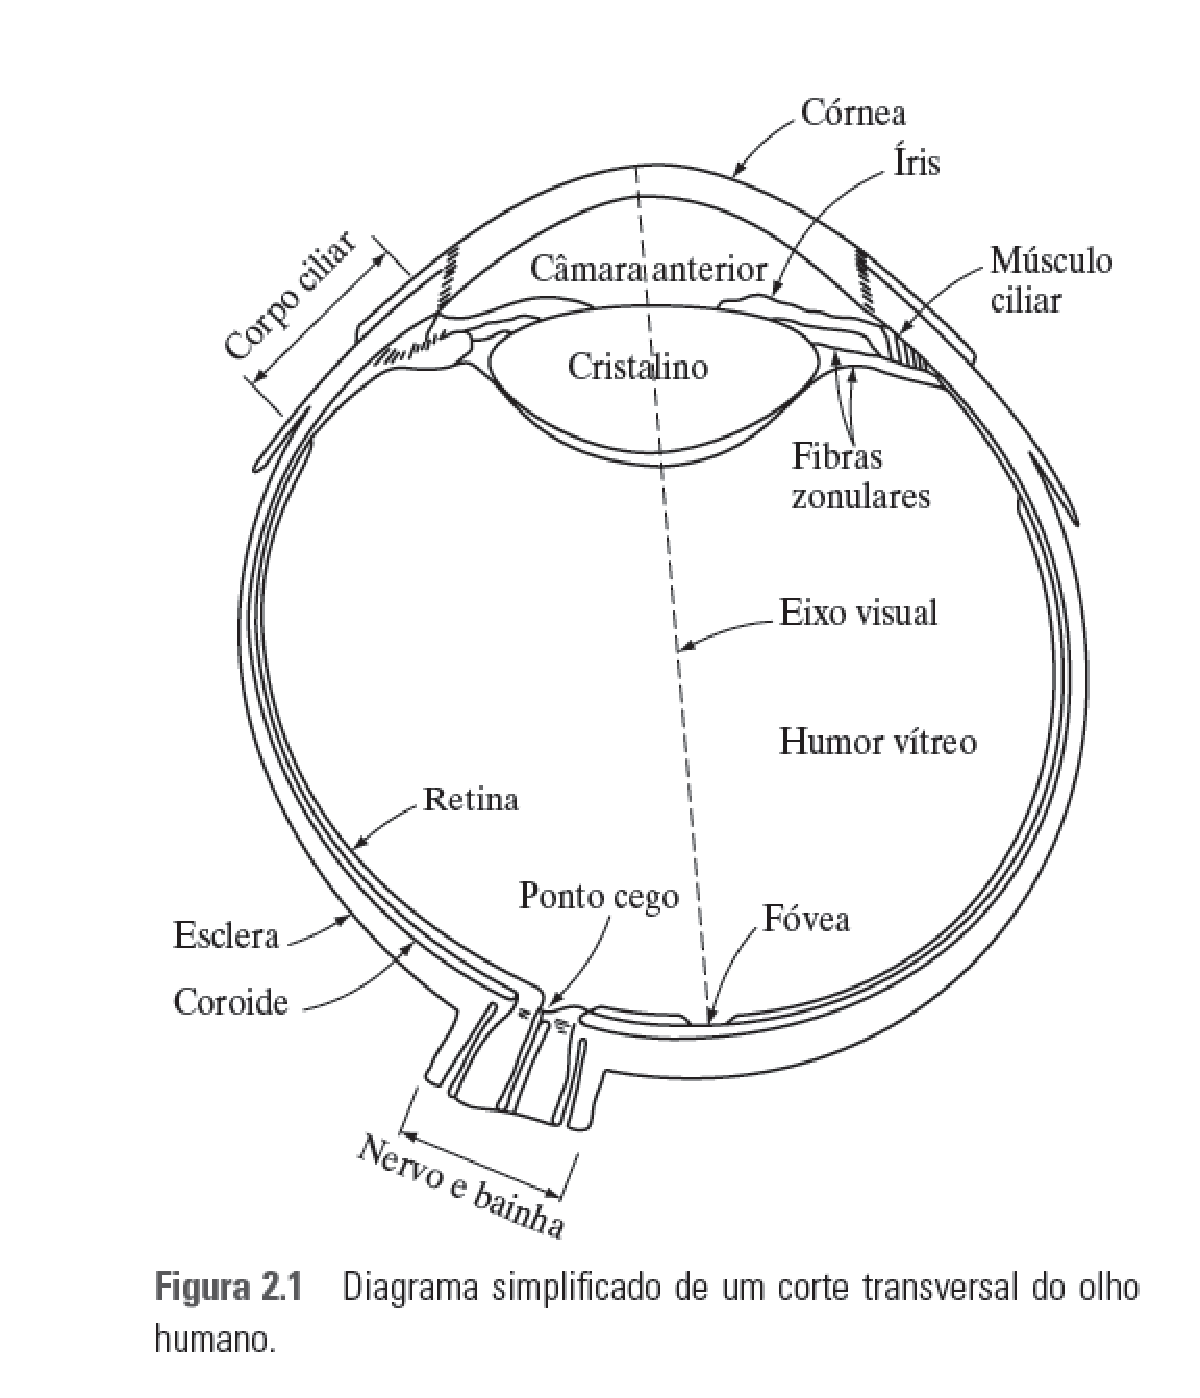
\includegraphics[width=1.0\textwidth]{figs/olho_gw}
         \end{center}
         }
      \end{slide}

%      \begin{slide}[toc=]{A estrutura do olho humano}
%         \begin{center}
%            \includegraphics[width=0.7\textwidth]{figs/olho_int}
%         \end{center}
%      \end{slide}

   \section[ slide = true]{A retina, cones e bastonetes}
      \begin{slide}[toc=]{Retina}
      \begin{itemize}
         \item Membrana mais interna do olho, formada por células fotossensíveis
         \item Dois tipos de fotorreceptores:
         \begin{itemize}
            \item Cones: 6 a 7 milhões, maior concentração na fóvea, visão fotópica (visão de luz clara),
            sensíveis à cor
            \item Bastonetes: 75 a 150 milhões, distribuídos mais uniformemente, visão escotópica (baixo
            nível de iluminação)
            \item Ponto cego:região de saída do nervo ótico, ausência de fotorreceptores
            \item Fóvea: centro da retina (337.000 cones, 150.000 cones por mm$^2$)
         \end{itemize}
      \end{itemize}
      \end{slide}   

      \begin{slide}[toc=]{Cones e bastonetes}
         \begin{center}
            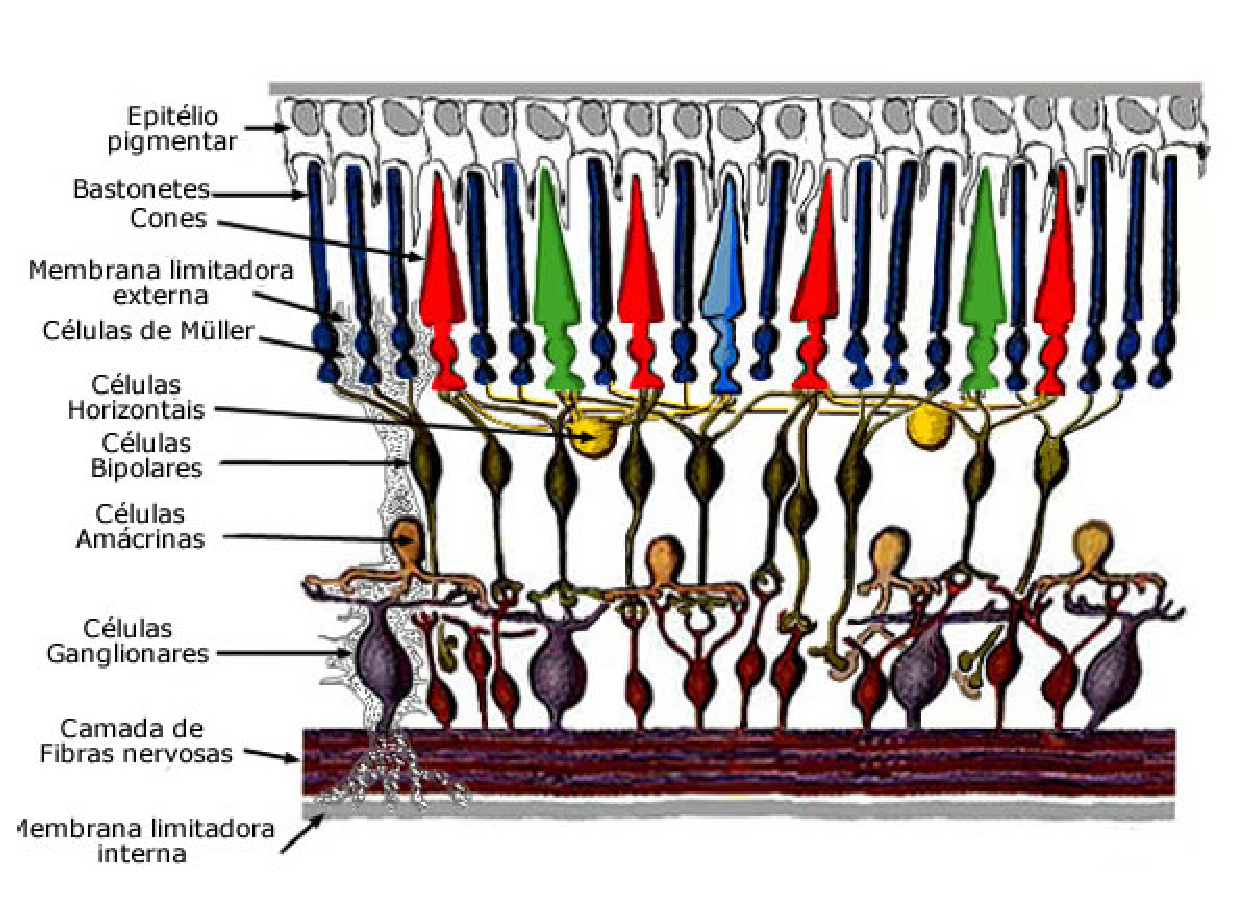
\includegraphics[height=.65\textheight]{figs/retina}
         %\end{center}
      %\end{slide}
      %\begin{slide}[toc=]{Cones e bastonetes}
      %   \begin{center}
            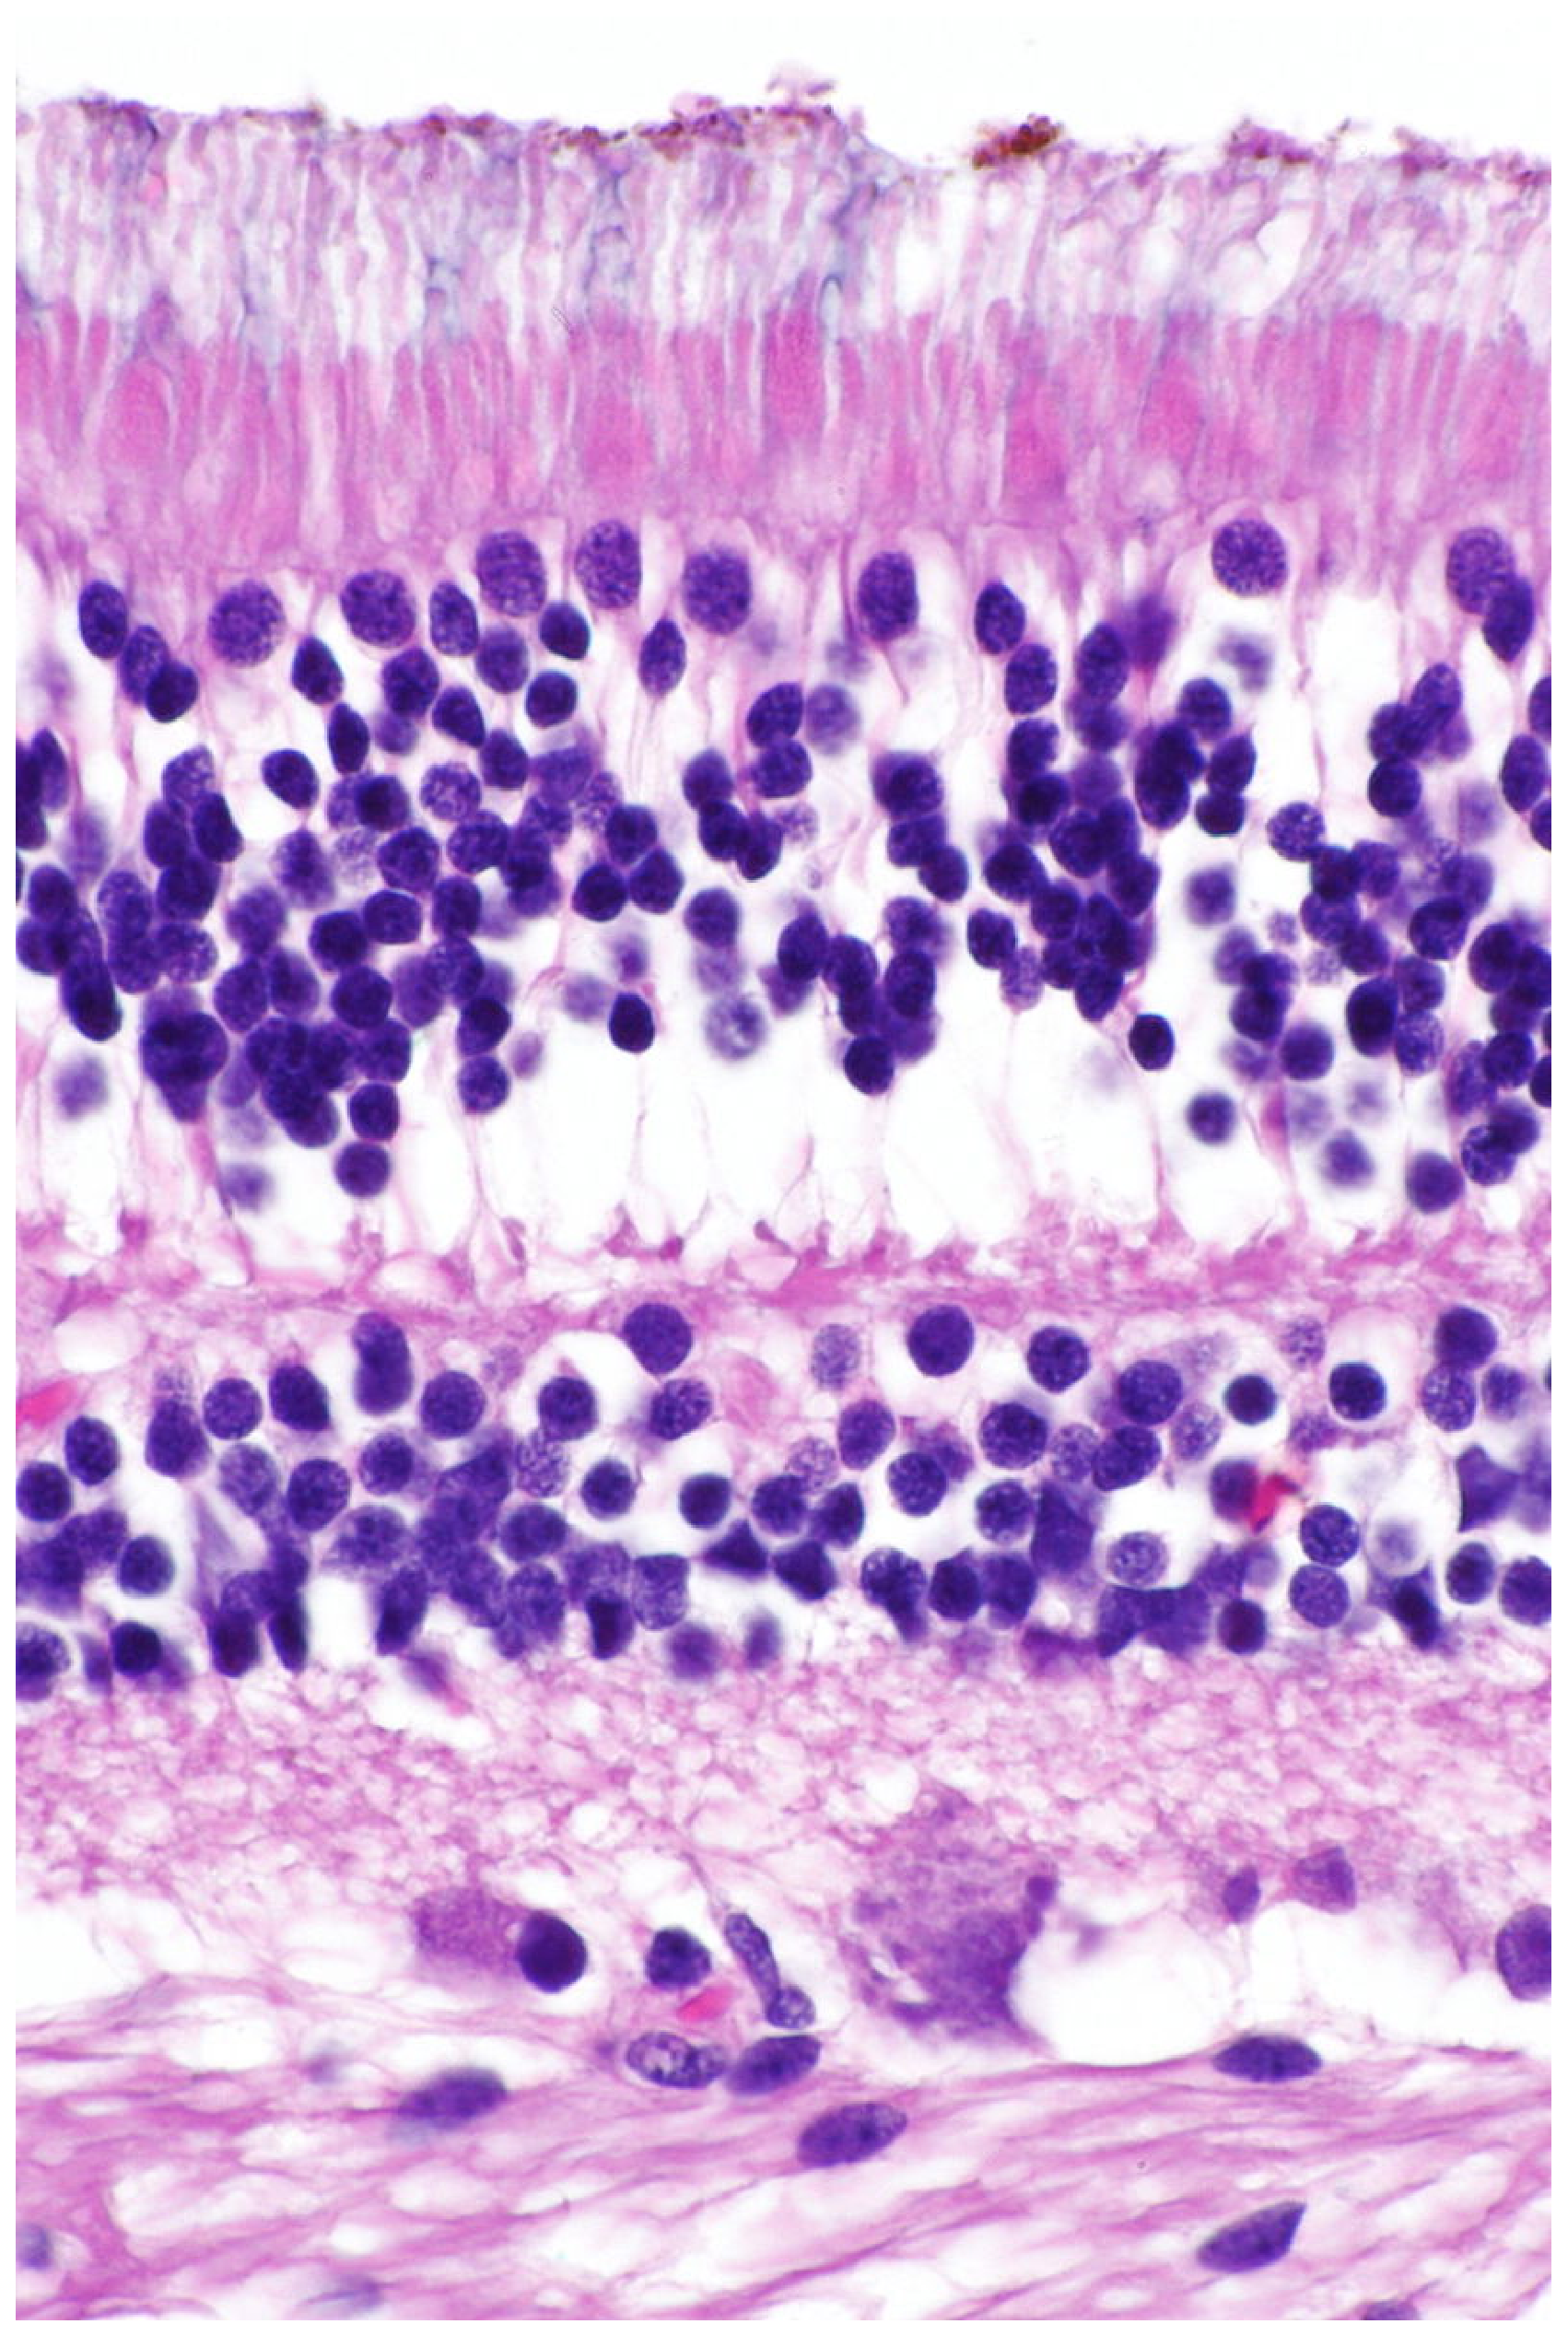
\includegraphics[height=.65\textheight]{figs/retina2}
         \end{center}
      \end{slide}

      \begin{slide}[toc=]{Distribuição de receptores}
         \begin{center}
            \includegraphics[width=1\textwidth]{figs/cb_gw}
         \end{center}
      \end{slide}
     
 %     \section[ slide = true]{Via visual}
  %     \begin{slide}[toc=]{Via visual}
   %       \begin{center}
    %         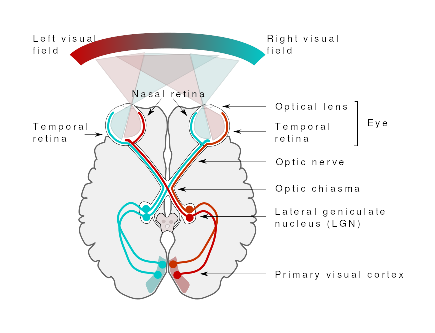
\includegraphics[width=.7\textwidth]{figs/visual_pathway}
     %     \end{center}
      % \end{slide}

      \begin{slide}[toc=]{Sensibilidade ao comprimento de onda}
         \begin{center}
            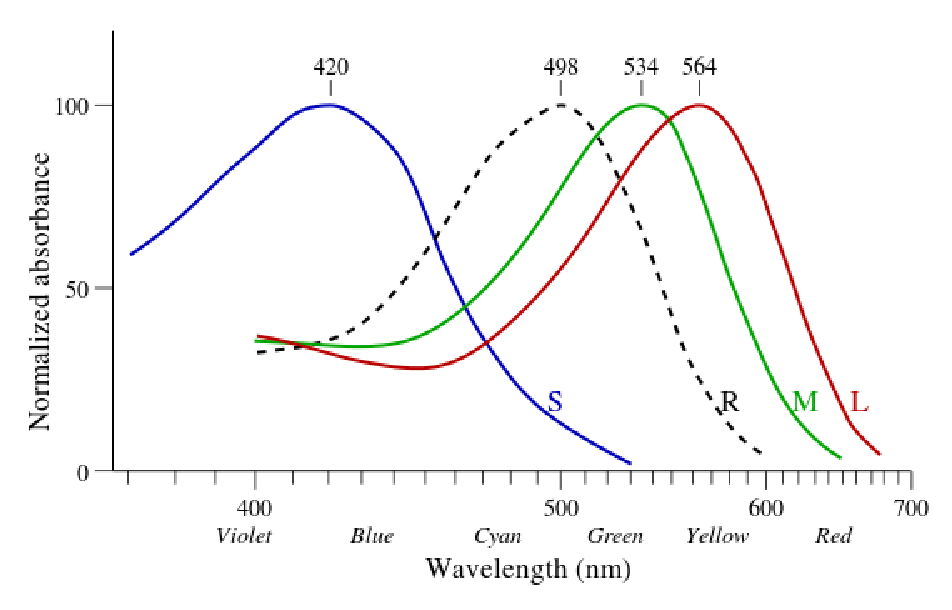
\includegraphics[width=.8\textwidth]{figs/cb_resp}
         \end{center}
      \end{slide}
      
     \section[ slide = true]{A luz e o espectro eletromagnético}
      \begin{slide}[toc=]{Banda visível}
         \begin{itemize}[type=1]
            \item Luz: radiação eletromagnética que pode ser vista
            \begin{center}
               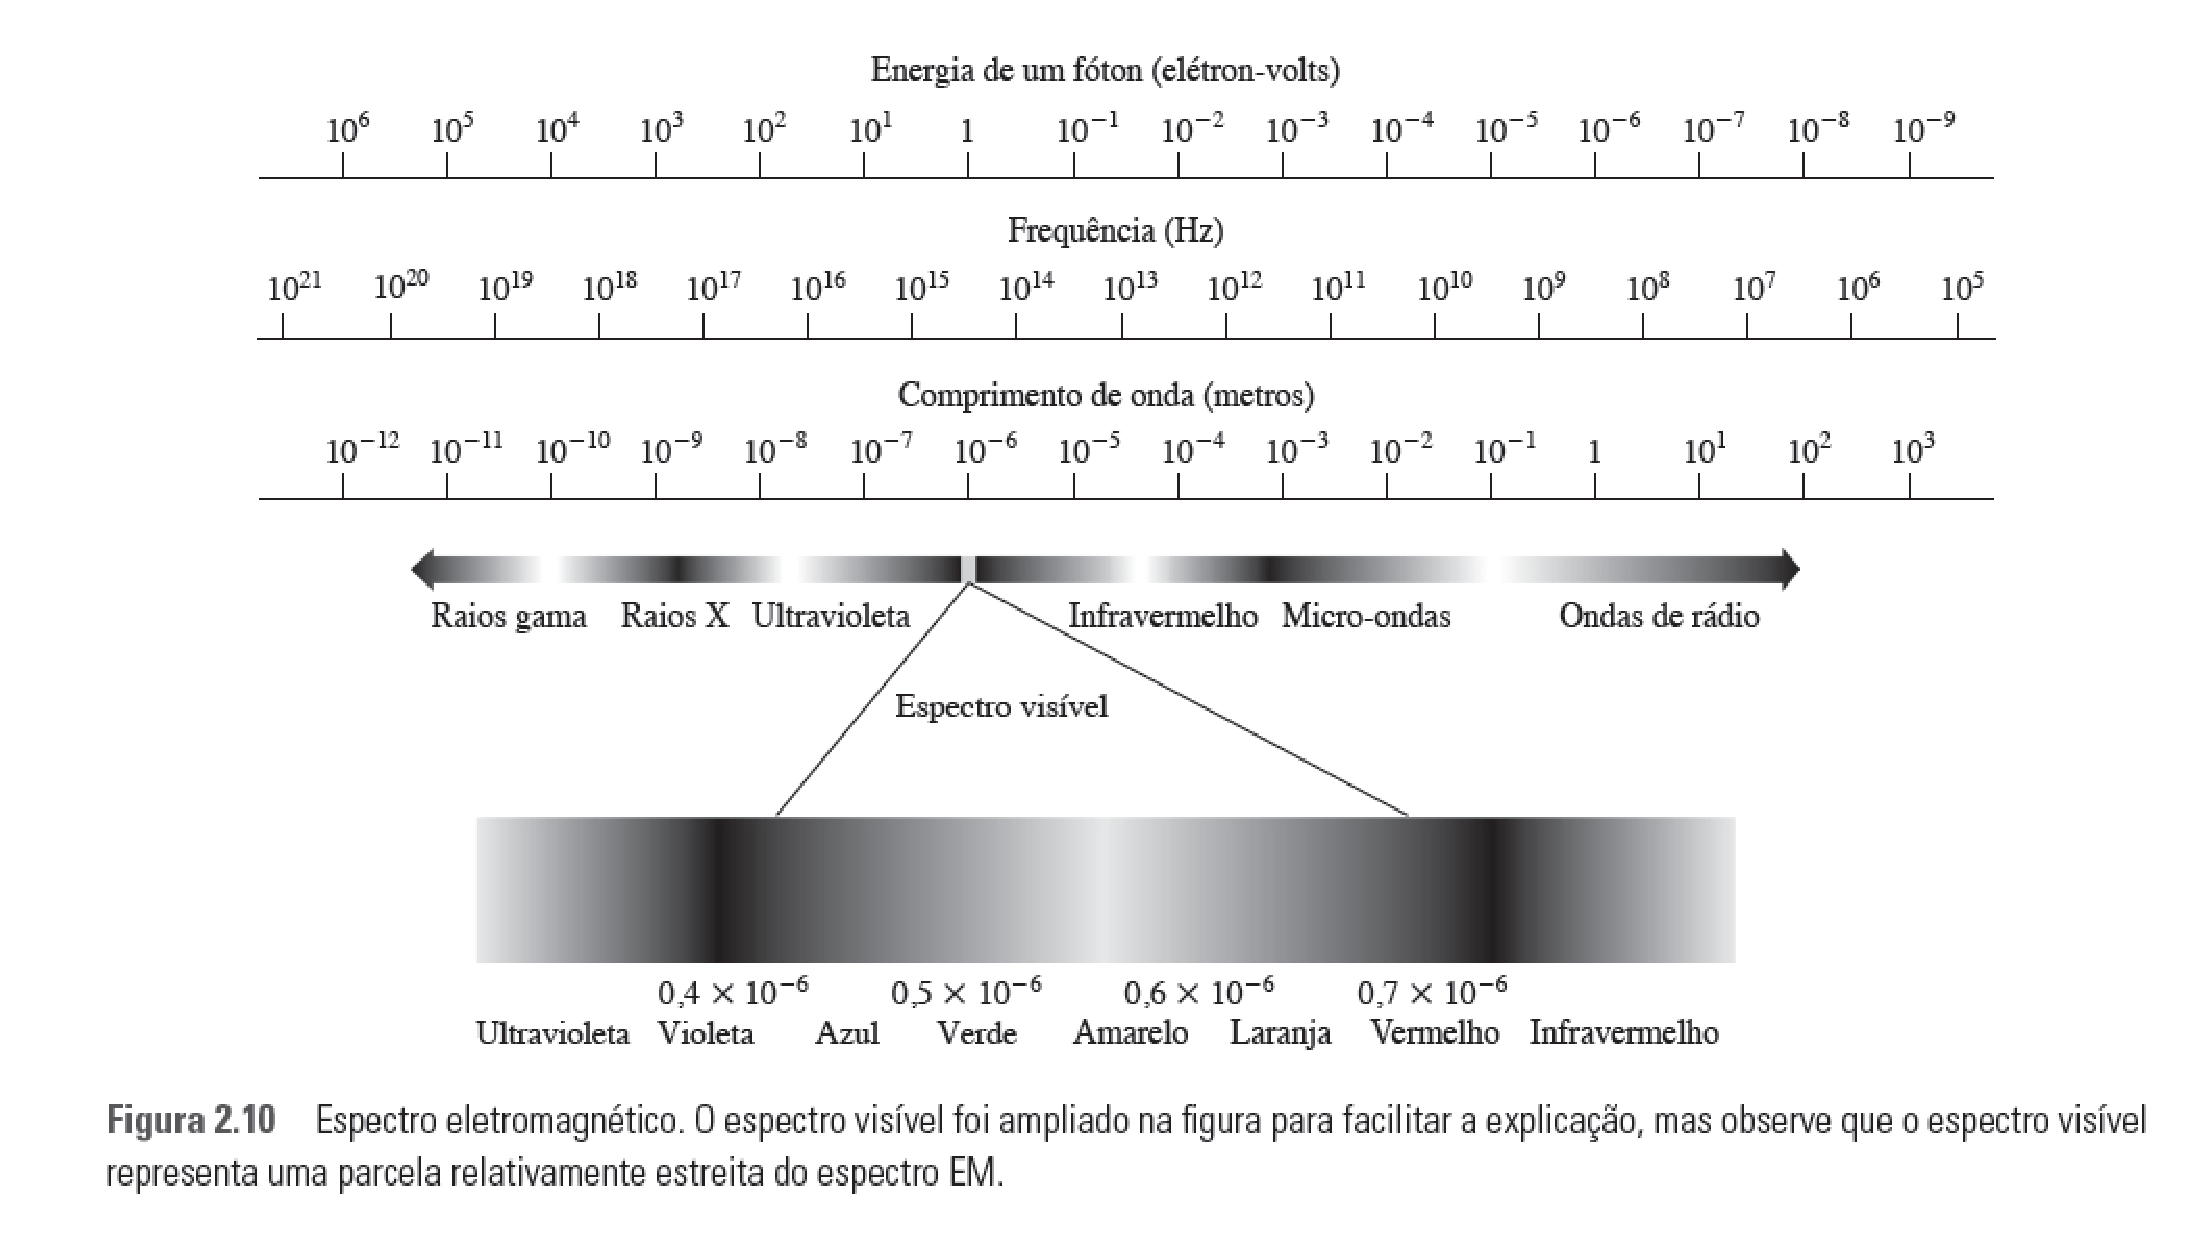
\includegraphics[width=.8\textwidth]{figs/fig0210}
            \end{center}
         \end{itemize}         
      \end{slide}
 
   \section[ slide = true]{Curiosidades da percepção visual}
  %     \begin{slide}[toc=]{Adaptação ao brilho e discriminação}
   %       \begin{itemize}
    %         \item Escala de níveis de intensidade: da ordem de $10^{10}$
     %        \item Brilho subjetivo: brilho percebido pelo SVH
      %       \item $B_a$: nível de adaptação ao brilho
       %      \item $B_b$: escala de brilho subjetivo adaptado a $B_a$
        %      \begin{itemize}
         %        \item Fenômenos de adaptação ao brilho
          %    \end{itemize}
           %  \begin{center}
            %    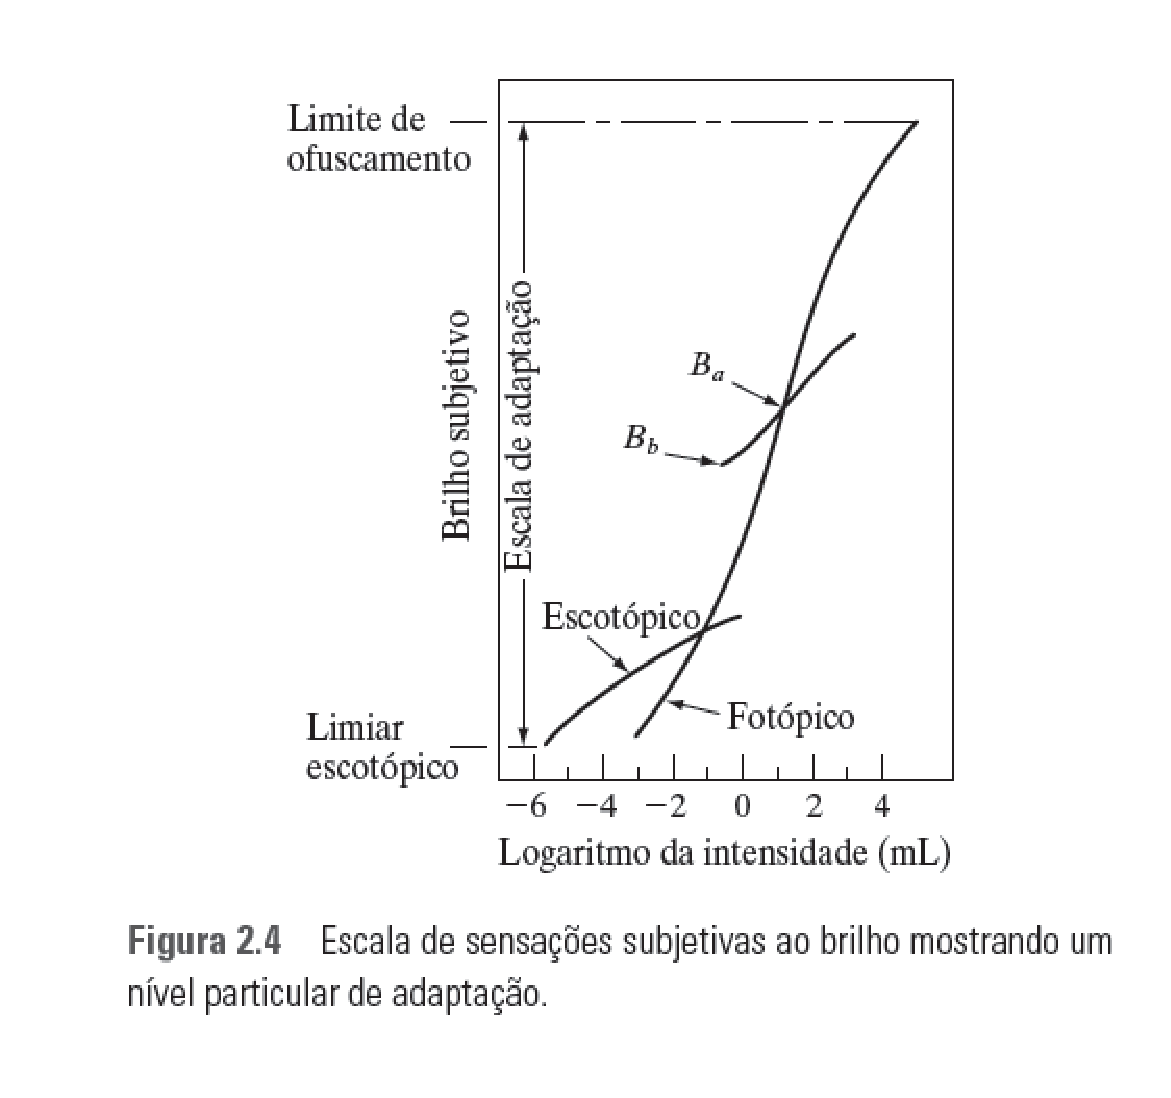
\includegraphics[width=0.35\textwidth]{figs/brilhosubjt}
  %           \end{center}
   %       \end{itemize}
    %   \end{slide}

      \begin{slide}[toc=]{Adaptação ao brilho e discriminação}
         \begin{itemize}
            \twocolumn{
            \item Caracterização de discriminação de brilho
            \begin{center}
               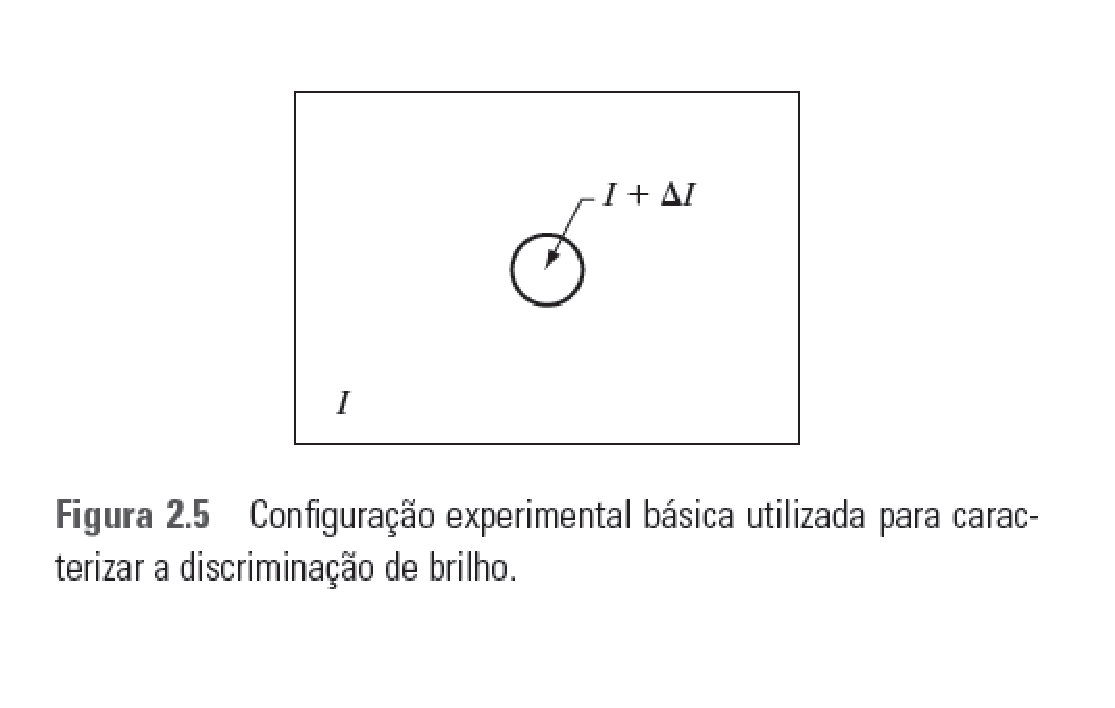
\includegraphics[width=1\textwidth]{figs/fig0205}
            \end{center}}
            {\item Razão de Weber
            \begin{center}
               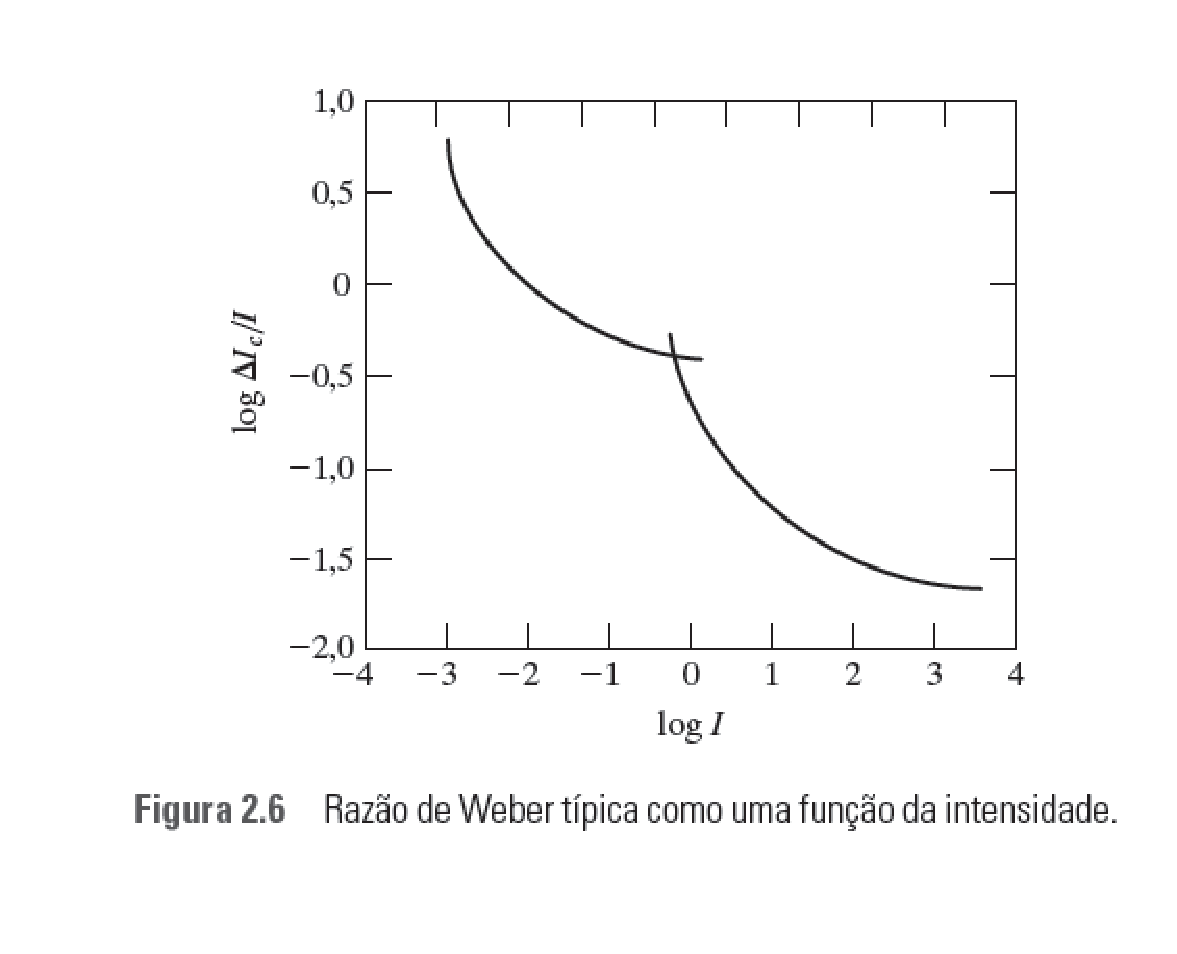
\includegraphics[width=1\textwidth]{figs/rweber_gw.eps}
            \end{center}}
            \item O que isso significa?\pause
            \begin{itemize}
               \item A percepção não depende apenas da intensidade em si, mas tembém do seu 
               entorno, do seu contexto
            \end{itemize}
         \end{itemize}
      \end{slide}

      \begin{slide}[toc=]{Adaptação ao brilho e discriminação}
         \begin{itemize}
            \item Bandas de Mach
            \begin{center}
               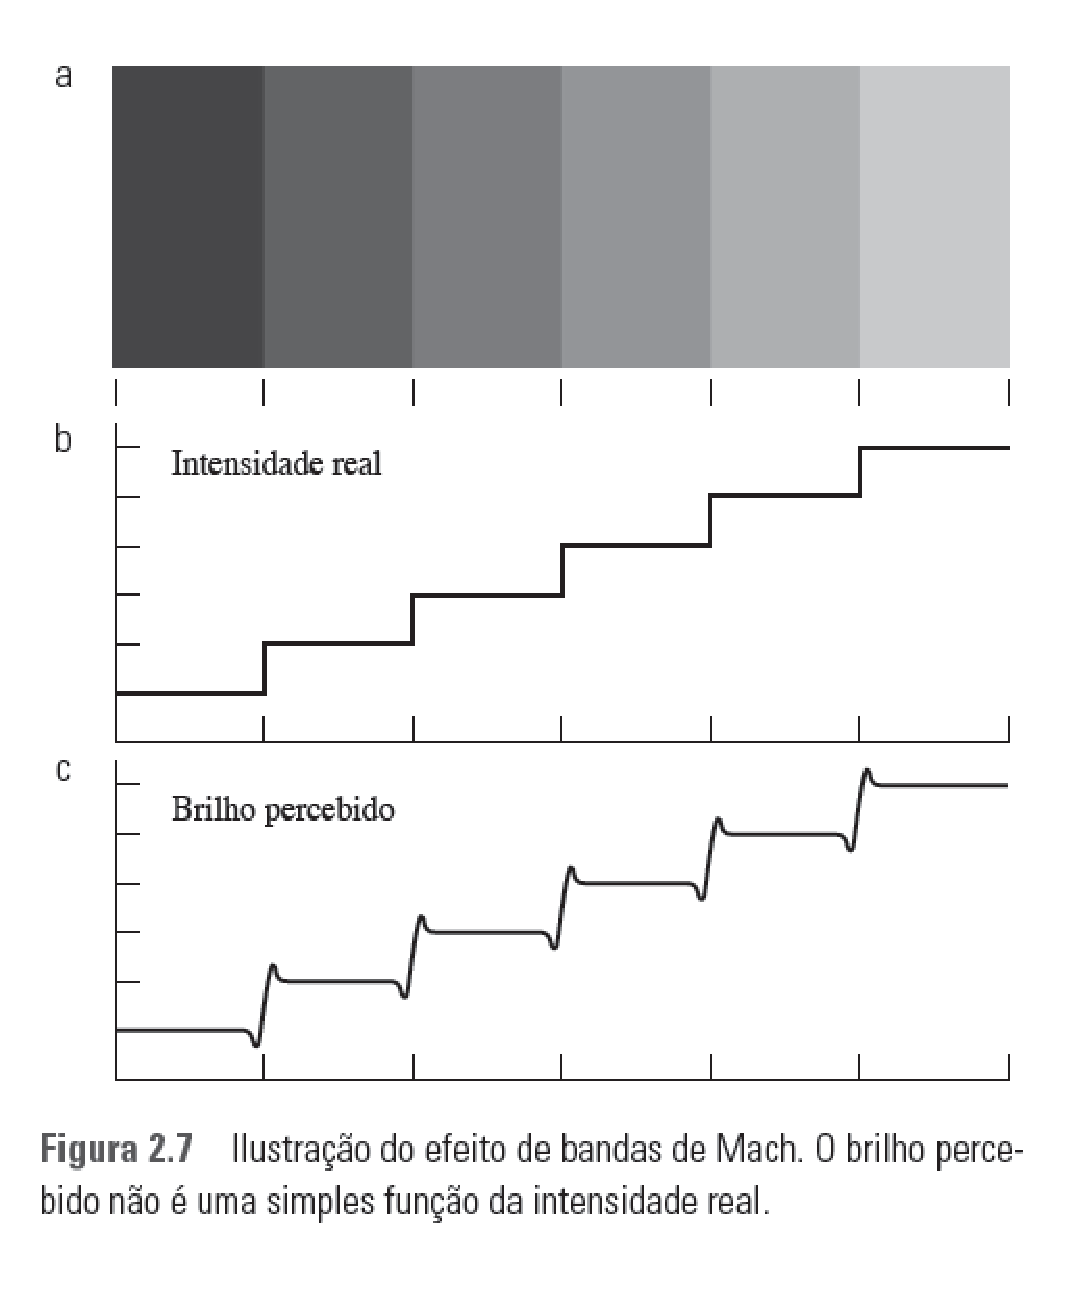
\includegraphics[width=0.4\textwidth]{figs/bmach_gw.eps}
            \end{center}
         \end{itemize}
      \end{slide}

      \begin{slide}[toc=]{Adaptação ao brilho e discriminação}
         \begin{itemize}
            \item Contraste simultâneo
            \begin{center}
               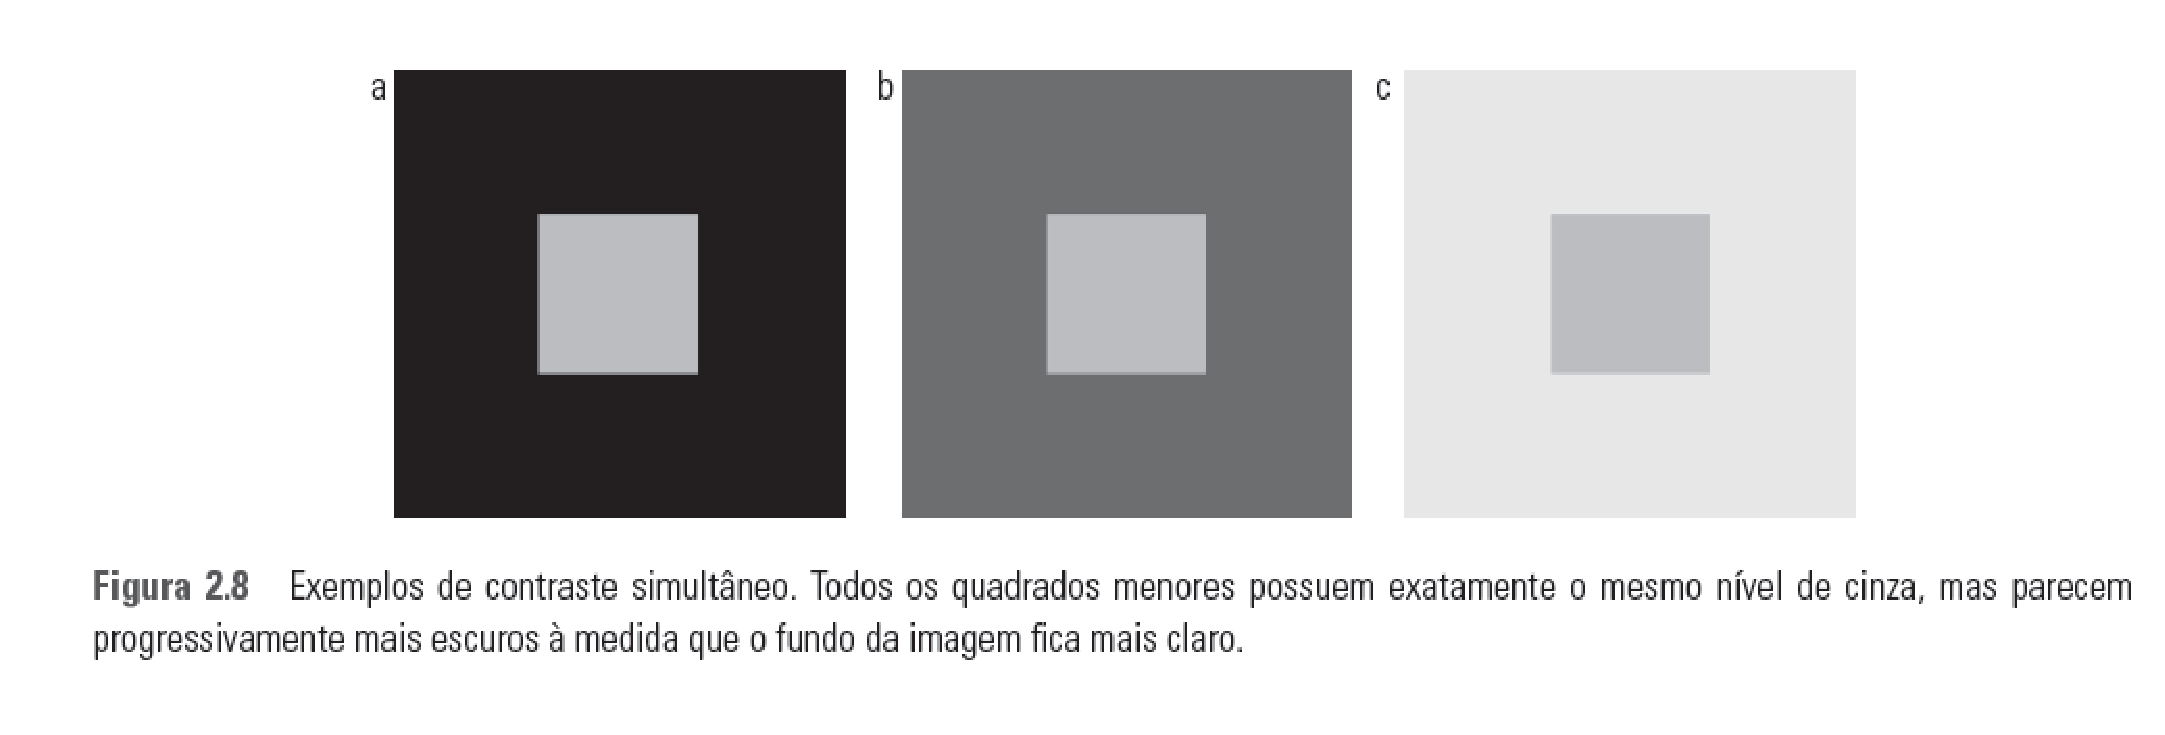
\includegraphics[width=\textwidth]{figs/csimul_gw.eps}
            \end{center}
         \end{itemize}
      \end{slide}

     
  %     \begin{slide}[toc=]{Outros conceitos}
   %       \begin{itemize}[type=1]
    %         \item Cores percebidas: luz refletida (filtrada) pelos corpos
     %        \item Luz sem cor, monocromática, acromática, ou escala de cinza: 
      %       luz cujo único atributo é a intensidade
       %      \item Radiância: quantidade total de energia emitida por uma fonte luminosa (W)
        %     \item Luminância: quantidade de energia percebida de uma fonte luminosa (lm)
         %    \item Brilho: descritor subjetivo da percepção da luz
          %\end{itemize}         
      % \end{slide}
      
      % \begin{slide}[toc=]{Efeitos interessantes: mudança de cor dos círculos}
       %      \begin{center}
        %        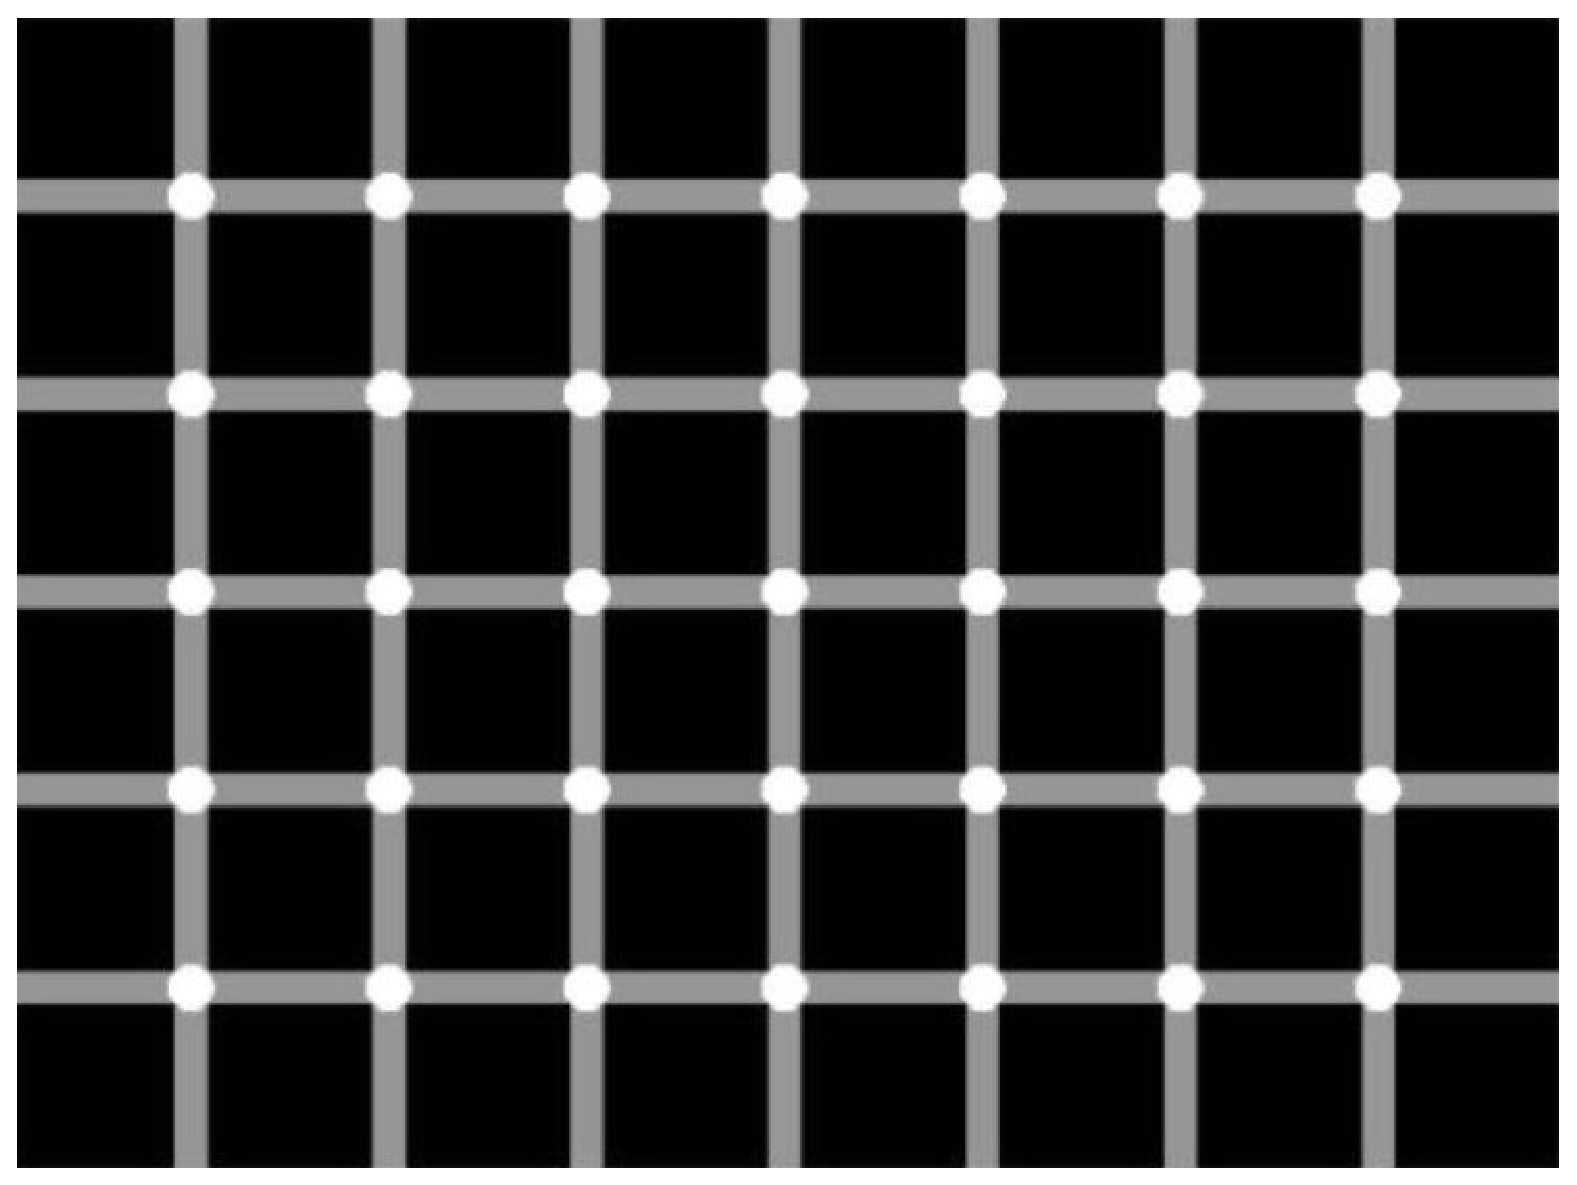
\includegraphics[height=0.8\textheight]{figs/2153774.eps}
         %    \end{center}
      % \end{slide}
      % \begin{slide}[toc=]{Efeitos interessantes: movimento aparente}
       %      \begin{center}
        %        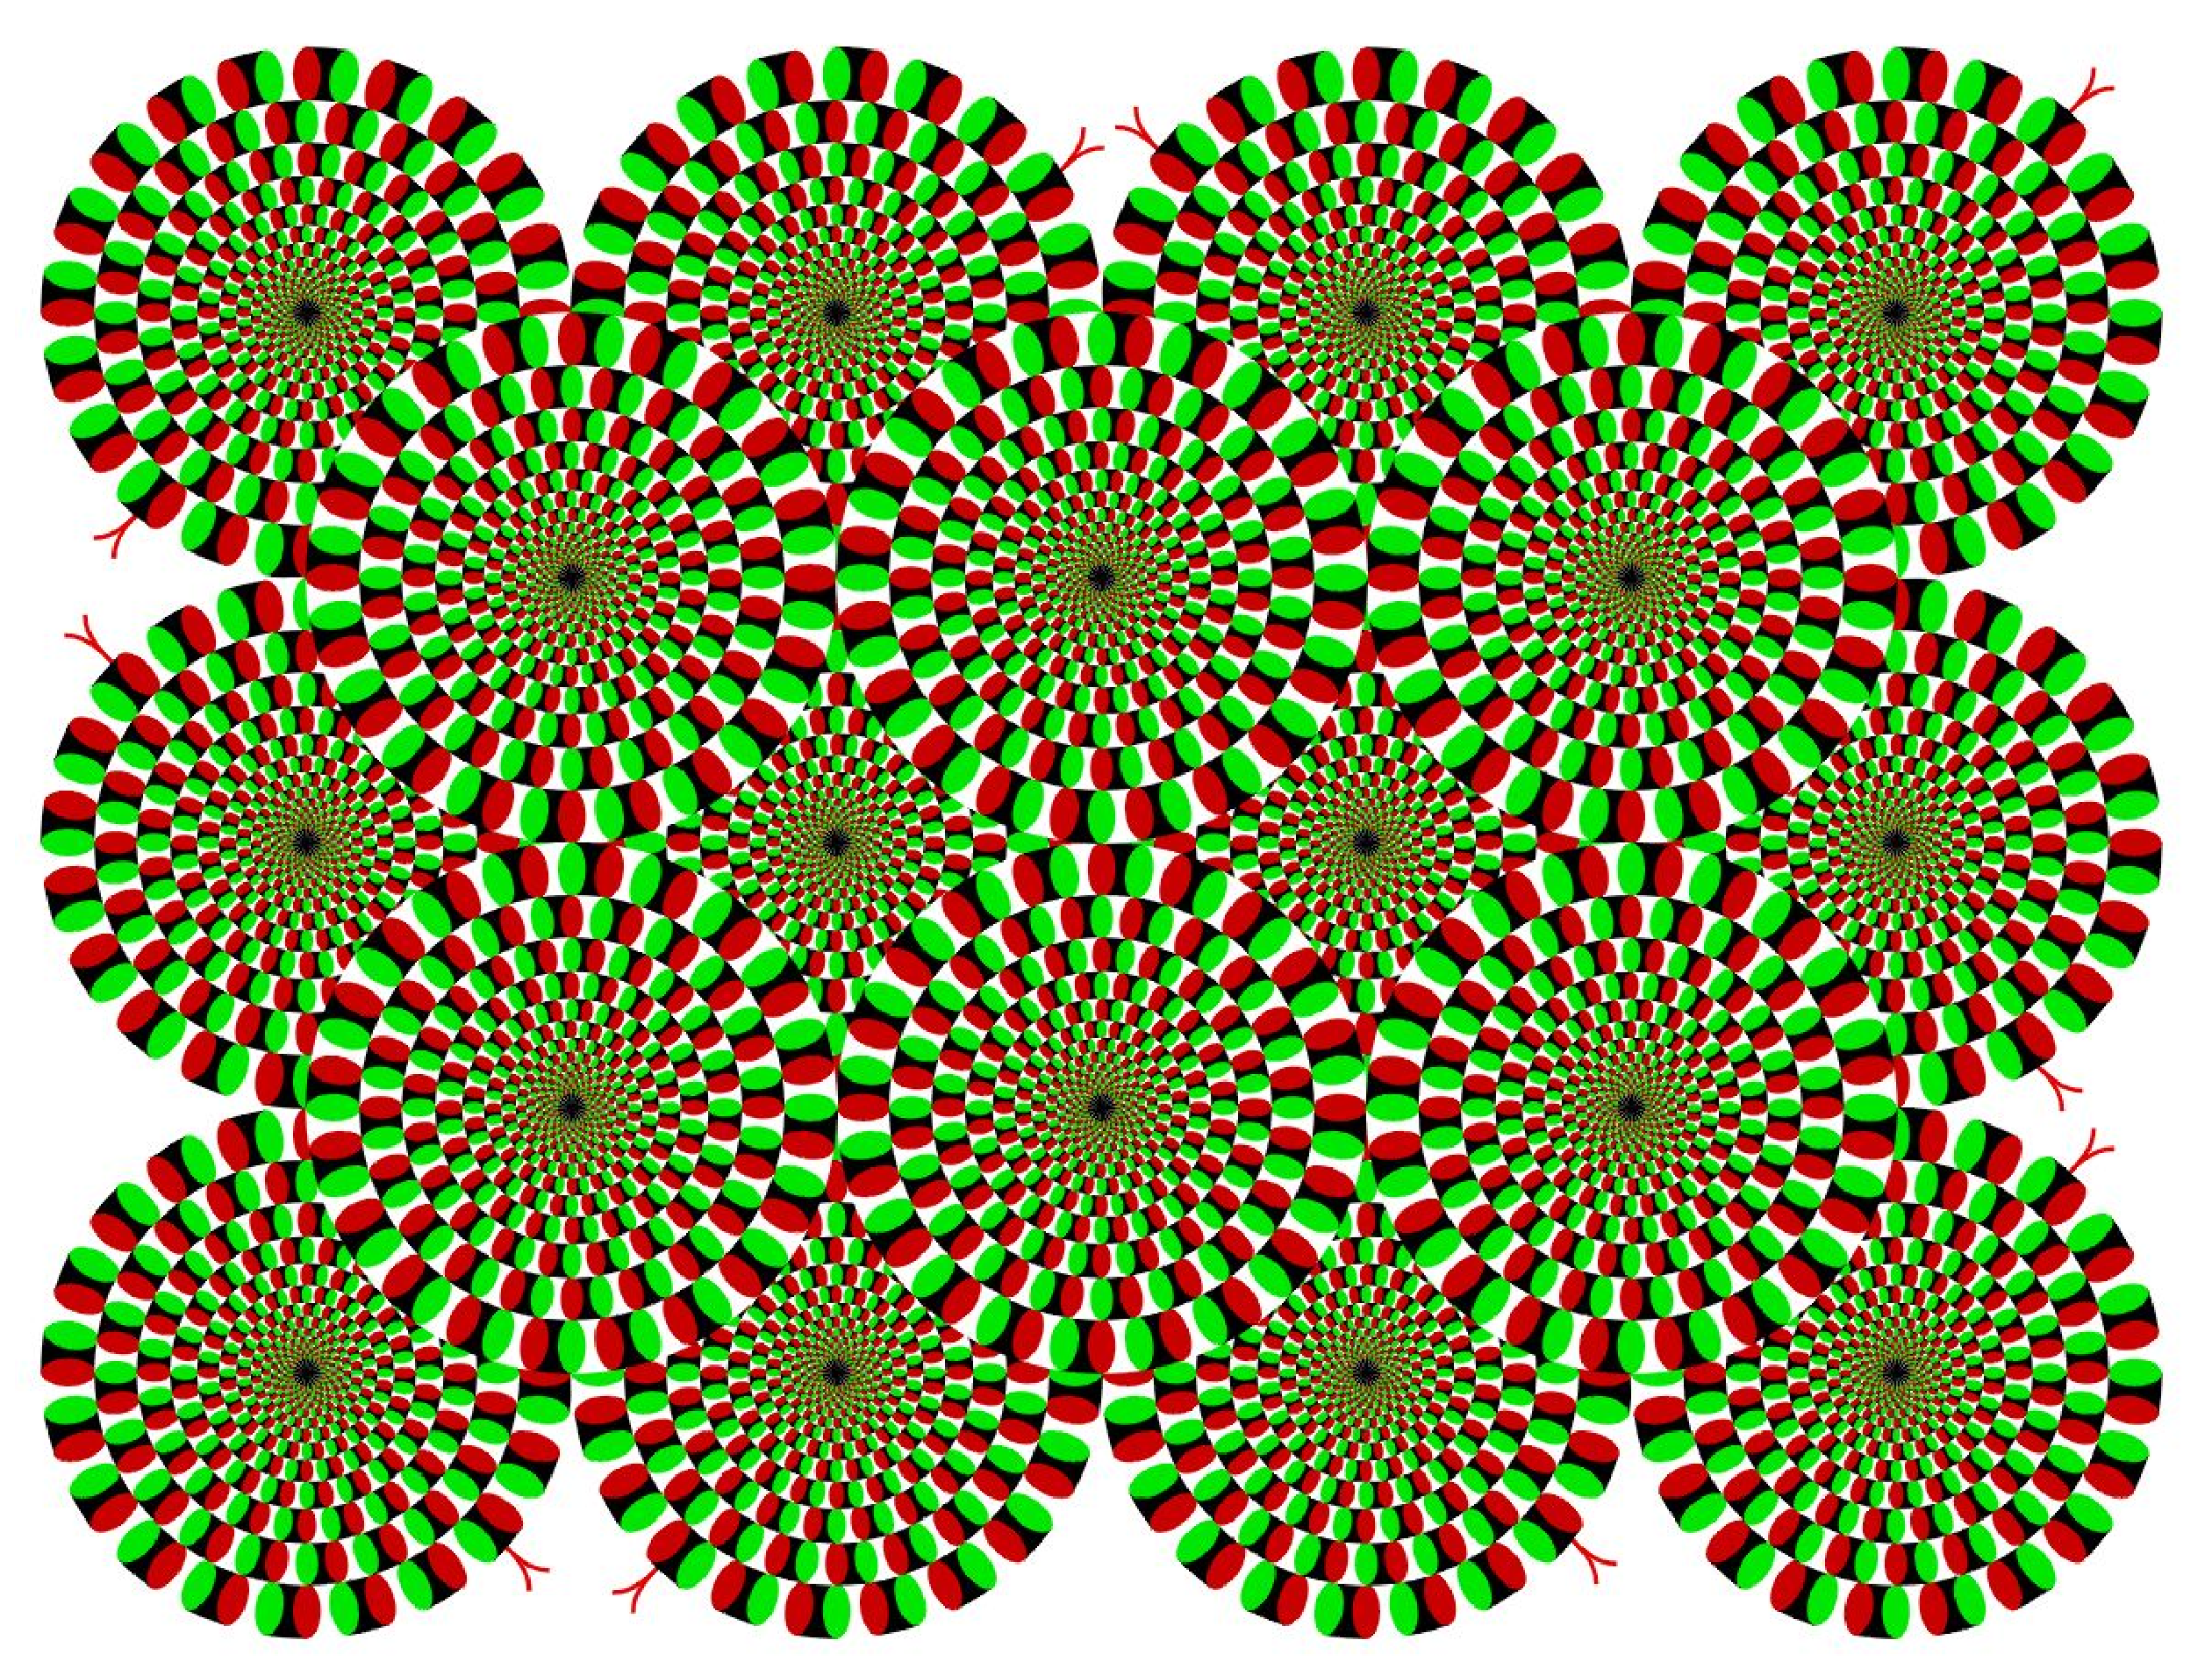
\includegraphics[height=0.8\textheight]{figs/2004071401_rotsnake7.eps}
         %    \end{center}
      % \end{slide}
      
      %\begin{slide}[toc=]{Efeitos interessantes}
      %      \begin{center}
      %         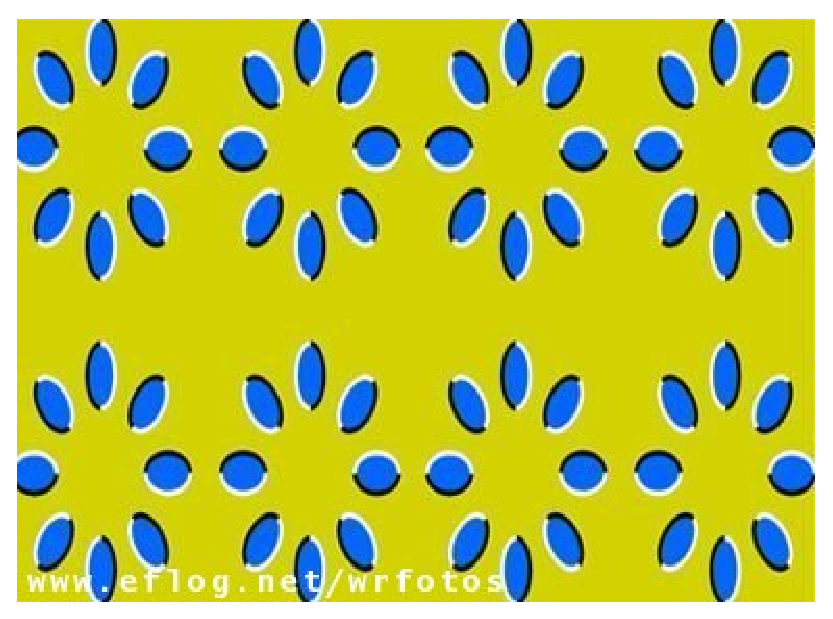
\includegraphics[height=0.8\textheight]{figs/img127904_wrfotos.eps}
      %      \end{center}
      %\end{slide}
%      \begin{slide}[toc=]{Efeitos interessantes: mudança de percepção devido ao contexto}
%            \begin{center}
%               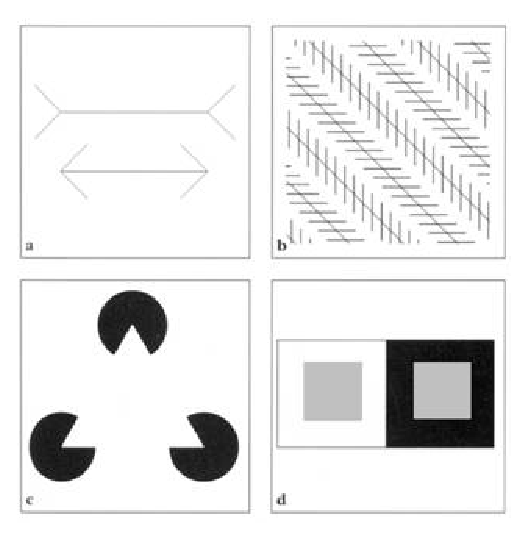
\includegraphics[height=0.8\textheight]{figs/image003.eps}
%            \end{center}
%      \end{slide}
%      \begin{slide}[toc=]{Efeitos interessantes: linhas paralelas?}
%            \begin{center}
%               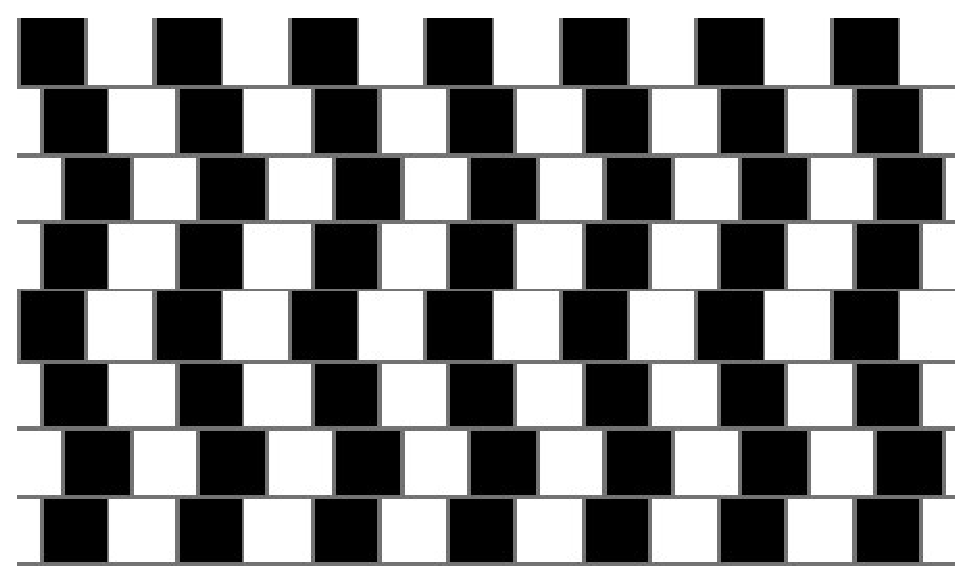
\includegraphics[height=0.8\textheight]{figs/parede.eps}
%            \end{center}
%      \end{slide}
      %\begin{slide}[toc=]{Efeitos interessantes}
      %      \begin{center}
      %         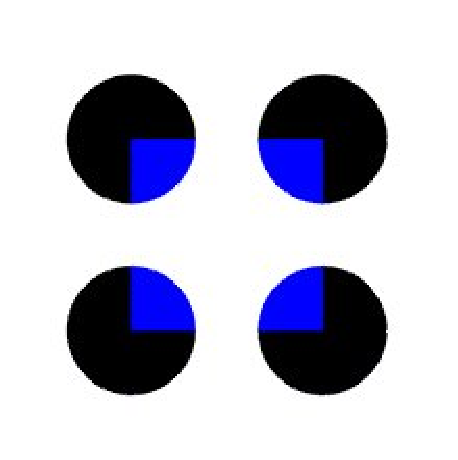
\includegraphics[height=0.8\textheight]{figs/quadrado_azul.eps}
      %      \end{center}
      %\end{slide}
      %\begin{slide}[toc=]{Efeitos interessantes}
      %      \begin{center}
      %         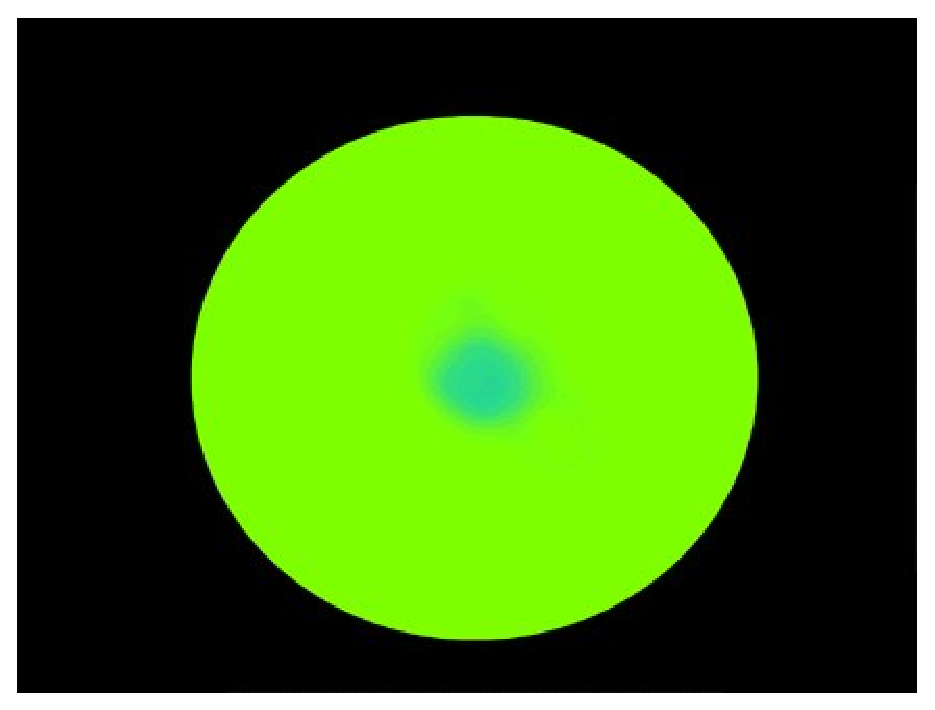
\includegraphics[height=0.8\textheight]{figs/bolaverde.eps}
      %      \end{center}
      %\end{slide}
%      \begin{slide}[toc=]{Efeitos interessantes: ponto cego}
%	    \vspace{5cm}
%            \begin{center}
%               
\includegraphics[width=0.8\textwidth]{figs/visao_22.eps}
%            \end{center}
%      \end{slide}
%      \begin{slide}[toc=]{Efeitos interessantes: aumento de carga cognitiva}
%            \begin{center}
%               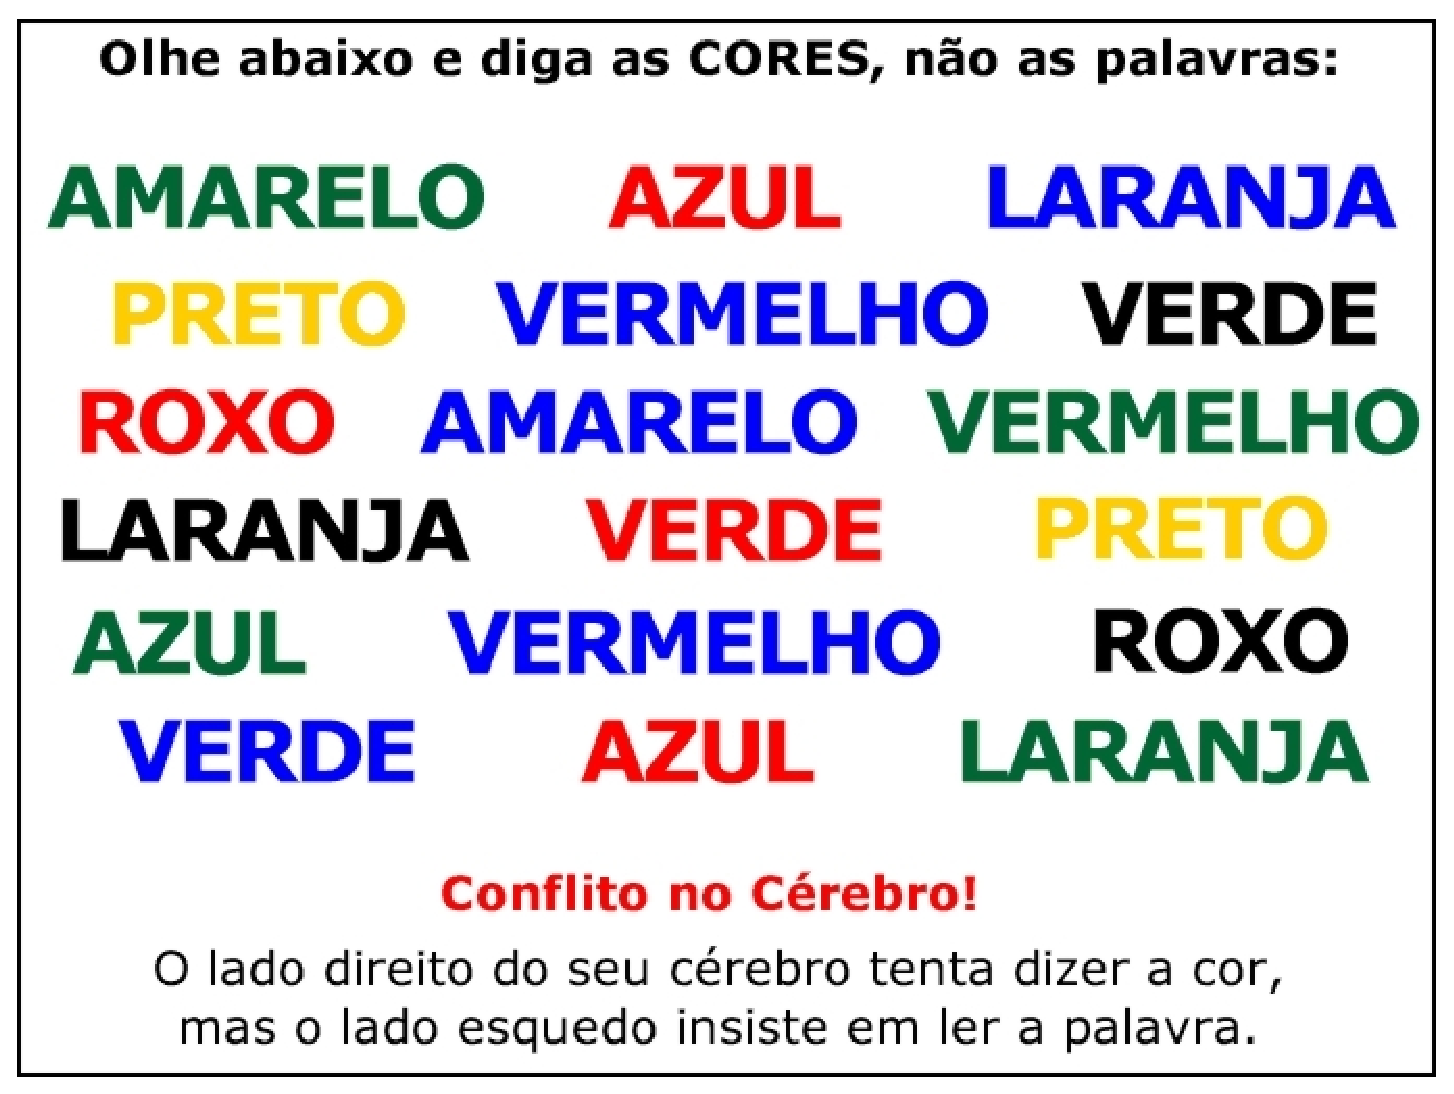
\includegraphics[height=0.8\textheight]{figs/conflito.eps}
%            \end{center}
%      \end{slide}
\end{document}
